% Preâmbulo (já tem graphicx e array no artigo; acrescente booktabs):
% \usepackage{graphicx}
% \usepackage{booktabs}
% \usepackage{array}
%
% Cabeçalho da coluna A: "A (points)" é a métrica de lesion reliance, em pontos de probabilidade.
% Valores: AUC = média das 4 redes; A = média das 4 redes (dados/chains_similar_auc.csv e dados/networks.csv).

\begin{table}[t]
\centering
\caption{Pipelines within $\pm0.01$ of the unfiltered AUC (mean of four networks): the two lowest and two highest in lesion reliance.}
\label{tab:chains}
% --- botões de tamanho e espaçamento ---
\footnotesize                       % tamanho do texto: \small > \footnotesize > \scriptsize
\setlength{\tabcolsep}{3pt}         % espaço horizontal entre colunas
\renewcommand{\arraystretch}{1.0}   % espaço vertical entre linhas (1.0 = mínimo; a altura da miniatura já separa)
\setlength{\abovecaptionskip}{4pt}  % espaço entre legenda e tabela (o padrão da classe é 10pt)
% larguras das colunas: miniatura | pipeline | AUC | A
\begin{tabular}{>{\centering\arraybackslash}m{0.7cm} m{6.4cm} >{\centering\arraybackslash}m{1.0cm} >{\centering\arraybackslash}m{1.5cm}}
    \toprule
    & \textbf{Pipeline} & \textbf{AUC} & \textbf{A (points)} \\
    \midrule
    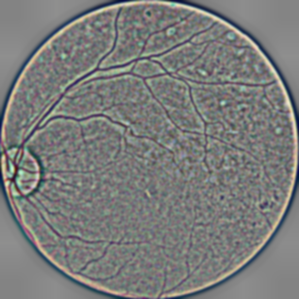
\includegraphics[width=0.6cm]{images/pipeline1.png}
    & Ben Graham $\rightarrow$ CLAHE $\rightarrow$ Gaussian
    & 0.903 & 4.2 \\

    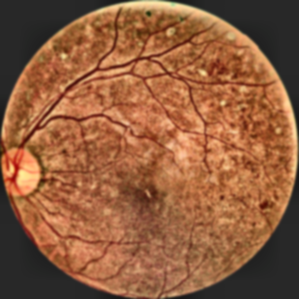
\includegraphics[width=0.6cm]{images/pipeline2.png}
    & AHE $\rightarrow$ Gaussian
    & 0.903 & 4.3 \\

    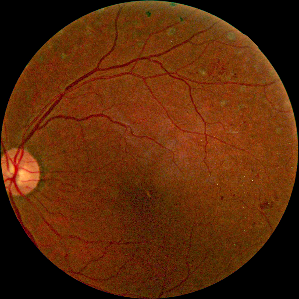
\includegraphics[width=0.6cm]{images/pipeline3.png}
    & Unfiltered
    & 0.910 & 9.1 \\

    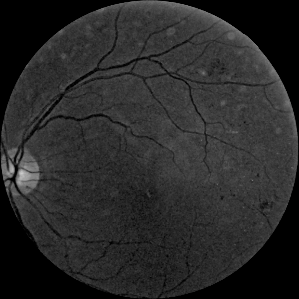
\includegraphics[width=0.6cm]{images/pipeline4.png}
    & LAB normaliz. $\rightarrow$ Green channel $\rightarrow$ Median
    & 0.901 & 12.7 \\

    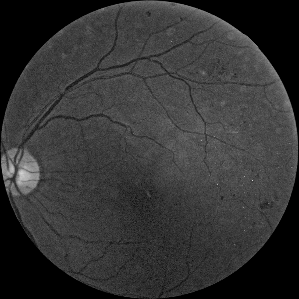
\includegraphics[width=0.6cm]{images/pipeline5.png}
    & LAB normaliz. $\rightarrow$ Grayscale
    & 0.904 & 14.1 \\
    \bottomrule
\end{tabular}
\end{table}
